\chapter{Introducción}
\graphicspath{ {img/chapter1/} {img/chapter4/} {img/chapter6/}}
\section{¿Qué es un motor gráfico?}
Un \textbf{motor gráfico} es un término que hace referencia a una serie de rutinas de programación que permiten el diseño, la creación y la representación de un videojuego. Del mismo modo existen motores de juegos que operan tanto en consolas de videojuegos como en sistemas operativos. A continuación se mostrarán dos ejemplos de videojuegos con distintos motores gráficos.

\begin{figure} [h]
  \centering
  \captionsetup[subfigure]{justification=centering}
  \begin{subfigure}{0.3\textwidth} 
    
\includegraphics[width=\textwidth]{supermario} 
    \caption{\textit{Super Mario Bros.} (1985)}
  \end{subfigure}
  \begin{subfigure}{0.3\textwidth}
    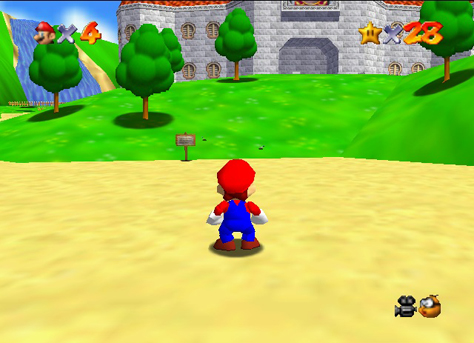
\includegraphics[width=\textwidth]{mario64} 
    \caption{\textit{Super Mario 64} (1996)}
  \end{subfigure}
  \caption{(a) utiliza un motor gráfico 2D (bidimensional) y (b) utiliza uno 3D (tridimensional) }
\end{figure}

El primer juego con un motor gráfico 3D en alcanzar un gran nivel de popularidad fue \textit{Doom} en 1993 y fue desarrollado mayoritariamente por John Carmack, jefe de programación en \textit{id Software}.

\newpage

\section{Introducción al Treball de Recerca}
Una revolución industrial consiste en la llegada de nuevas máquinas y métodos que permiten optimizar los procesos de producción. La industria del software está pasando actualmente por una de estas revoluciones, dónde están surgiendo multitud de herramientas para agilizar la producción. Estas herramientas oscilan desde librerías\footnote{Colección de recursos no volátiles utilizados por programas informáticos.} para funciones matemáticas simples, pasando por editores de texto inteligentes que van acompañados por un compilador y depurador (\textit{IDE}s) e incluso llegan a motores gráficos comerciales disponibles a cualquier programador con una habilidad intermedia, permitiendo saltar uno de los pasos más laboriosos del proceso de creación de videojuegos.

La llegada de esta ola ha sido bastante polémica y ha dividido a las comunidades. Por una parte no se puede negar la importancia de tener herramientas más potentes. Pero por la otra parte hay muchos que piensan que esto ha llevado a la gente a no preocuparse por algunas cuestiones sólo porque lo ven como una cosa del pasado, un problema menor que ya está solucionado por la herramienta que usan. Estos problemas terminan por acumularse y pueden desencadenar en problemas mayores si no se intentan solventar desde la raíz.

Mi opinión siempre ha sido la de permanecer escéptico a los programas que pretenden tener un uso generalizado, y siempre he creído que cada herramienta es para una situación concreta, y no se puede intentar usar el mismo método y herramientas para todo.

\section{Objetivos}
Según la prioridad asignada he separado los objetivos en dos categorías. Es importante recordar que \textbf{no es un objetivo} obtener un producto de una complejidad y rendimiento similar a librerías y motores gráficos comerciales.
\subsection{Objetivos principales}
\begin{itemize}
\item Investigar la factibilidad de desarrollar una librería gráfica.
\item Estudiar la factibilidad de desarrollar un motor gráfico.
\item Comprender el funcionamiento de un motor gráfico a nivel interno.
\item Crear un motor gráfico que funcione en cualquier sistema operativo.
\item Familiarizarse con herramientas de expresión científica.
\end{itemize} 
\subsection{Objetivos secundarios}
\begin{itemize}
\item Permitir la compilación\footnote{Traducción de un programa escrito en lenguaje de programación a un lenguaje que el ordenador puede entender.} tanto de la librería gráfica como del motor en cualquier entorno de desarrollo.
\item Comparar la librería gráfica propia con ejemplos comerciales.
\item Comparar el motor gráfico creado con ejemplos comerciales.
\end{itemize}


\section{Motivación personal}
Existen una gran cantidad de motivaciones personales alrededor del proyecto. Por una parte soy un gran fanático de la computación y con el Treball de Recerca tengo una buena oportunidad de hacer algo que siempre he deseado hacer. También me he inspirado por un videojuego llamado \textit{Handmade Hero}, el cuál está siendo desarrollado, como hace referencia el nombre, \textit{a mano}, sin hacer uso de librerías modernas. También tengo interés en hacer un programa de un tamaño mayor a lo que estoy acostumbrado y aprender a organizar y a documentar el proceso. Además pretendo aprender a usar diversas herramientas para redactar textos científicos, como el propio lenguaje en el que está escrito este documento, \LaTeX\footnote{Sistema de preparación de documentos ampliamente utilizado en la comunidad cientificoténcnica.}, y el editor de texto Emacs.

\section{Relevancia del estudio en el campo}
Como he comentado previamente, en la actualidad existe una gran polémica con respecto a este tema. Muchas empresas de la indústria de los videojuegos han decidido abandonar la creación de motores para uso específico de sus videojuegos en pro de adoptar motores comerciales generales. Esta decisión ha traído muchos escándalos en los que estos motores de uso generalizado funcionan terriblemente mal en algunas configuraciones concretas y debido a la naturaleza cerrada del motor la desarrolladora del videojuego no ha podido solucionar el problema.

Independientemente de la rentabilidad de desarrollar un motor gráfico en la época actual, algo que es indudable es que es completamente necesario entender el funcionamiento del mismo, para poder extraer el máximo rendimiento posible, sea tanto un motor \textit{hecho a mano} como uno comercial.

\section{Límites del trabajo}
Está clara la inviabilidad de desarrollar un motor gráfico a la altura de los ofrecidos acutalmente en el mercado, pues estos han estado desarrollados por un equipo de expertos durante años y tienden a ofrecer una cantidad de rendimiento y funcionalidad que duramente se puede replicar en un proyecto hecho en unos meses por alguien que no tiene ni las nociones académicas ni la experiencia ni los recursos necesarios. Sin embargo esto sólo significa que mi producto no será de uso a la indústria, pero puede tener valor académico.

\section{Metodología empleada para realizar la investigación}
El método del trabajo consiste en la creación de un motor gráfico con una funcionalidad limitada pero suficiente para elaborar una conclusión y reconsiderar la hipótesis. No sólo se intentará hacer un motor gráfico sino que además se busca replicar la funcionalidad de OpenGL\footnote{Librería gráfica muy popular por su flexibilidad y rendimiento.} en una librería gráfica desarrollada paralelamente al motor gráfico para poder ir un paso más allá. La hipótesis será revisada tanto por el resultado final del proceso de elaboración del motor como por la investigación en el funcionamiento de la industria de los motores gráficos.

\section{Hipótesis}
\textit{Los equipos de desarrollo de software deberían de aspirar a ser ellos mismos quienes crean las herramientas que utilizarán para crear el software en sí. En caso de que esta sea una decisión no rentable, su máxima prioridad debería de ser entender cómo funcionan las herramientas que utilizarán.}


Considero que cuando uno forma parte del proceso de creación de software, tiene que tener el mayor conocimiento posible del funcionamiento de aquello que está haciendo. Eso significa psar por pasos que muchas veces se saltan con la finalidad de agilizar el proceso, no obstante no creo que esto sea positivo ya que ha llevado a serioes problemas a la larga.
